% Timbangan dua lengan untuk konsep persamaan linear
% Seluruh koordinat dihitung dari geometri: lengan horizontal, piringan di ujung lengan.
\documentclass[tikz,border=6pt]{standalone}
\usepackage{amsmath}
\definecolor{bg}{HTML}{171D2B}
\definecolor{acc}{HTML}{F7B538}
\definecolor{dish}{HTML}{8FA6C4}
\pagecolor{bg}
\begin{document}
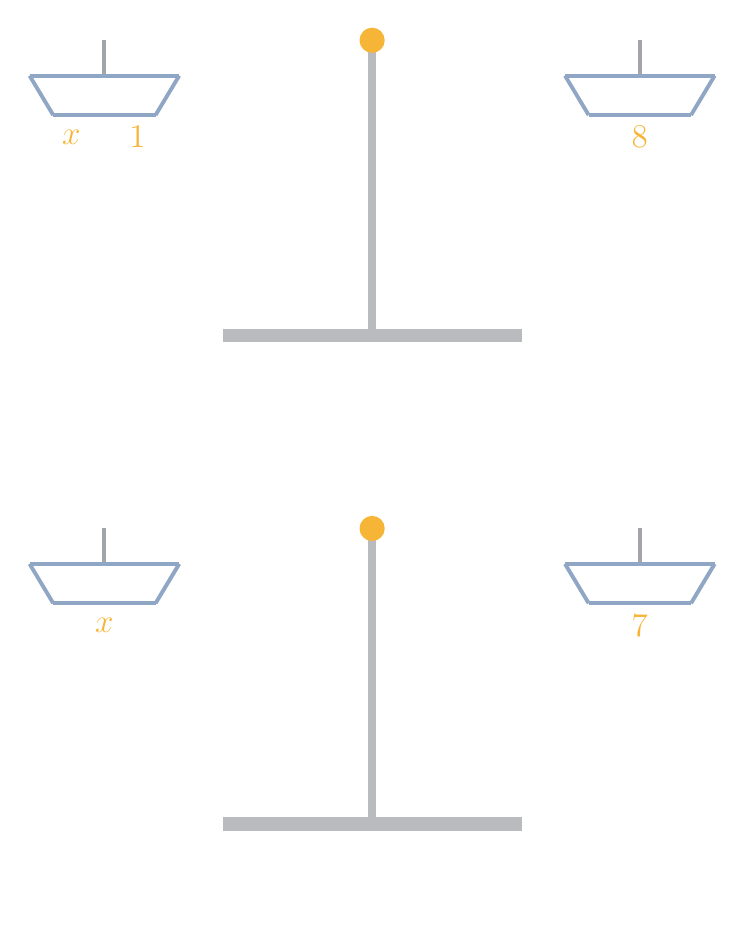
\begin{tikzpicture}[line width=1.4pt, text=white, x=1cm, y=1cm]

% ====== TIMBANGAN SEIMBANG ======
\def\bxA{-3.4}   % ujung kiri lengan
\def\tx{0}       % titik tengah
\def\bxB{3.4}    % ujung kanan lengan
\def\ary{2.6}    % tinggi lengan
\def\dis{0.45}   % jarak piringan di bawah ujung lengan

% tiang & alas
\draw[white!70!bg, line width=3pt] (\tx,\ary) -- (\tx,-1.15);
\draw[white!70!bg, line width=3pt] (-1.5,-1.15) -- (1.5,-1.15);
\draw[white!70!bg, line width=5pt] (-1.9,-1.15) -- (1.9,-1.15);

% lengan dan penggantung
\draw[white, line width=2pt] (\bxA,\ary) -- (\bxB,\ary);
\fill[acc] (\tx,\ary) circle (0.16);
\draw[white!60!bg] (\bxA,\ary) -- (\bxA,\ary-\dis);
\draw[white!60!bg] (\bxB,\ary) -- (\bxB,\ary-\dis);

% piringan kiri: "x" dan "1"  (dua blok bertumpuk, ukuran sama)
\draw[dish] (\bxA-0.95,\ary-\dis) -- (\bxA+0.95,\ary-\dis);
\draw[dish] (\bxA-0.95,\ary-\dis) -- (\bxA-0.65,\ary-\dis-0.5);
\draw[dish] (\bxA+0.95,\ary-\dis) -- (\bxA+0.65,\ary-\dis-0.5);
\draw[dish] (\bxA-0.65,\ary-\dis-0.5) -- (\bxA+0.65,\ary-\dis-0.5);
\node[acc, font=\large] at (\bxA-0.42,\ary-\dis-0.78) {$x$};
\node[acc, font=\large] at (\bxA+0.42,\ary-\dis-0.78) {$1$};

% piringan kanan: blok besar "8"
\draw[dish] (\bxB-0.95,\ary-\dis) -- (\bxB+0.95,\ary-\dis);
\draw[dish] (\bxB-0.95,\ary-\dis) -- (\bxB-0.65,\ary-\dis-0.5);
\draw[dish] (\bxB+0.95,\ary-\dis) -- (\bxB+0.65,\ary-\dis-0.5);
\draw[dish] (\bxB-0.65,\ary-\dis-0.5) -- (\bxB+0.65,\ary-\dis-0.5);
\node[acc, font=\large] at (\bxB,\ary-\dis-0.78) {$8$};

% keterangan keseimbangan
\node[white, font=\normalsize] at (0,-2.1) {$x+1=8 \;\Rightarrow\; x=7$};

% ====== TIMBANGAN SETELAH KEDUA LEMBU DIKURANGI 1 ======
\begin{scope}[shift={(0,-6.2)}]
\draw[white!70!bg, line width=3pt] (\tx,\ary) -- (\tx,-1.15);
\draw[white!70!bg, line width=3pt] (-1.5,-1.15) -- (1.5,-1.15);
\draw[white!70!bg, line width=5pt] (-1.9,-1.15) -- (1.9,-1.15);

\draw[white, line width=2pt] (\bxA,\ary) -- (\bxB,\ary);
\fill[acc] (\tx,\ary) circle (0.16);
\draw[white!60!bg] (\bxA,\ary) -- (\bxA,\ary-\dis);
\draw[white!60!bg] (\bxB,\ary) -- (\bxB,\ary-\dis);

% piringan kiri: hanya "x"
\draw[dish] (\bxA-0.95,\ary-\dis) -- (\bxA+0.95,\ary-\dis);
\draw[dish] (\bxA-0.95,\ary-\dis) -- (\bxA-0.65,\ary-\dis-0.5);
\draw[dish] (\bxA+0.95,\ary-\dis) -- (\bxA+0.65,\ary-\dis-0.5);
\draw[dish] (\bxA-0.65,\ary-\dis-0.5) -- (\bxA+0.65,\ary-\dis-0.5);
\node[acc, font=\large] at (\bxA,\ary-\dis-0.78) {$x$};

% piringan kanan: "7"
\draw[dish] (\bxB-0.95,\ary-\dis) -- (\bxB+0.95,\ary-\dis);
\draw[dish] (\bxB-0.95,\ary-\dis) -- (\bxB-0.65,\ary-\dis-0.5);
\draw[dish] (\bxB+0.95,\ary-\dis) -- (\bxB+0.65,\ary-\dis-0.5);
\draw[dish] (\bxB-0.65,\ary-\dis-0.5) -- (\bxB+0.65,\ary-\dis-0.5);
\node[acc, font=\large] at (\bxB,\ary-\dis-0.78) {$7$};

\node[white, font=\normalsize] at (0,-2.1) {$x+1-1=8-1 \;\Rightarrow\; x=7$};
\end{scope}

\end{tikzpicture}
\end{document}
